\documentclass[journal,12pt,twocolumn]{IEEEtran}

\usepackage{setspace}
\usepackage{gensymb}
\singlespacing
\usepackage[cmex10]{amsmath}
\usepackage{float}
\usepackage{amsthm}

\usepackage{mathrsfs}
\usepackage{txfonts}
\usepackage{stfloats}
\usepackage{bm}
\usepackage{cite}
\usepackage{cases}
\usepackage{subfig}

\usepackage{longtable}
\usepackage{multirow}

\usepackage{enumitem}
\usepackage{mathtools}
\usepackage{steinmetz}
\usepackage{tikz}
\usepackage{circuitikz}
\usepackage{verbatim}
\usepackage{tfrupee}
\usepackage[breaklinks=true]{hyperref}
\usepackage{graphicx}
\usepackage{tkz-euclide}

\usetikzlibrary{calc,math}
\usepackage{listings}
    \usepackage{color}                                            %%
    \usepackage{array}                                            %%
    \usepackage{longtable}                                        %%
    \usepackage{calc}                                             %%
    \usepackage{multirow}                                         %%
    \usepackage{hhline}                                           %%
    \usepackage{ifthen}                                           %%
    \usepackage{lscape}     
\usepackage{multicol}
\usepackage{chngcntr}
\usepackage{float}
\DeclareMathOperator*{\Res}{Res}

\renewcommand\thesection{\arabic{section}}
\renewcommand\thesubsection{\thesection.\arabic{subsection}}
\renewcommand\thesubsubsection{\thesubsection.\arabic{subsubsection}}

\renewcommand\thesectiondis{\arabic{section}}
\renewcommand\thesubsectiondis{\thesectiondis.\arabic{subsection}}
\renewcommand\thesubsubsectiondis{\thesubsectiondis.\arabic{subsubsection}}


\hyphenation{op-tical net-works semi-conduc-tor}
\def\inputGnumericTable{}                                 %%

\lstset{
%language=C,
frame=single, 
breaklines=true,
columns=fullflexible
}
\begin{document}


\newtheorem{theorem}{Theorem}[section]
\newtheorem{problem}{Problem}
\newtheorem{proposition}{Proposition}[section]
\newtheorem{lemma}{Lemma}[section]
\newtheorem{corollary}[theorem]{Corollary}
\newtheorem{example}{Example}[section]
\newtheorem{definition}[problem]{Definition}

\newcommand{\BEQA}{\begin{eqnarray}}
\newcommand{\EEQA}{\end{eqnarray}}
\newcommand{\define}{\stackrel{\triangle}{=}}
\bibliographystyle{IEEEtran}
\raggedbottom
\setlength{\parindent}{0pt}
\providecommand{\mbf}{\mathbf}
\providecommand{\pr}[1]{\ensuremath{\Pr\left(#1\right)}}
\providecommand{\qfunc}[1]{\ensuremath{Q\left(#1\right)}}
\providecommand{\sbrak}[1]{\ensuremath{{}\left[#1\right]}}
\providecommand{\lsbrak}[1]{\ensuremath{{}\left[#1\right.}}
\providecommand{\rsbrak}[1]{\ensuremath{{}\left.#1\right]}}
\providecommand{\brak}[1]{\ensuremath{\left(#1\right)}}
\providecommand{\lbrak}[1]{\ensuremath{\left(#1\right.}}
\providecommand{\rbrak}[1]{\ensuremath{\left.#1\right)}}
\providecommand{\cbrak}[1]{\ensuremath{\left\{#1\right\}}}
\providecommand{\lcbrak}[1]{\ensuremath{\left\{#1\right.}}
\providecommand{\rcbrak}[1]{\ensuremath{\left.#1\right\}}}
\theoremstyle{remark}
\newtheorem{rem}{Remark}
\newcommand{\sgn}{\mathop{\mathrm{sgn}}}
\providecommand{\abs}[1]{\left\vert#1\right\vert}
\providecommand{\res}[1]{\Res\displaylimits_{#1}} 
\providecommand{\norm}[1]{\left\lVert#1\right\rVert}
%\providecommand{\norm}[1]{\lVert#1\rVert}
\providecommand{\mtx}[1]{\mathbf{#1}}
\providecommand{\mean}[1]{E\left[ #1 \right]}
\providecommand{\fourier}{\overset{\mathcal{F}}{ \rightleftharpoons}}
%\providecommand{\hilbert}{\overset{\mathcal{H}}{ \rightleftharpoons}}
\providecommand{\system}{\overset{\mathcal{H}}{ \longleftrightarrow}}
	%\newcommand{\solution}[2]{\textbf{Solution:}{#1}}
\newcommand{\solution}{\noindent \textbf{Solution: }}
\newcommand{\cosec}{\,\text{cosec}\,}
\providecommand{\dec}[2]{\ensuremath{\overset{#1}{\underset{#2}{\gtrless}}}}
\newcommand{\myvec}[1]{\ensuremath{\begin{pmatrix}#1\end{pmatrix}}}
\newcommand{\mydet}[1]{\ensuremath{\begin{vmatrix}#1\end{vmatrix}}}
\numberwithin{equation}{subsection}
\makeatletter
\@addtoreset{figure}{problem}
\makeatother
\let\StandardTheFigure\thefigure
\let\vec\mathbf
\renewcommand{\thefigure}{\theproblem}
\def\putbox#1#2#3{\makebox[0in][l]{\makebox[#1][l]{}\raisebox{\baselineskip}[0in][0in]{\raisebox{#2}[0in][0in]{#3}}}}
     \def\rightbox#1{\makebox[0in][r]{#1}}
     \def\centbox#1{\makebox[0in]{#1}}
     \def\topbox#1{\raisebox{-\baselineskip}[0in][0in]{#1}}
     \def\midbox#1{\raisebox{-0.5\baselineskip}[0in][0in]{#1}}
\vspace{3cm}
\title{CBSE Maths 10, 2007}
%\author{Peri Priyanka$^{*}$
\author{Peri Priyanka
	\thanks{}
}
\maketitle
\newpage
\tableofcontents
\bigskip
\renewcommand{\thefigure}{\theenumi}
\renewcommand{\thetable}{\theenumi}
Get Python codes from 
%
\begin{lstlisting}
https://github.com/gadepall/cbse-papers/2007/math/10/solutions/codes
\end{lstlisting}
%
Get latex-tikz codes from 
%
\begin{lstlisting}
https://github.com/gadepall/cbse-papers/2007/math/10/solutions
\end{lstlisting}
\section{Discrete maths}
\renewcommand{\theequation}{\theenumi}
\begin{enumerate}[label=\thesection.\arabic*.,ref=\thesection.\theenumi]
\numberwithin{equation}{enumi}
\item If X +K is the GCD of $ X^2-2X-15 $ and $X^3+27$, find the value of K.\\
\solution consider the given equations,
\begin{align}
& X^2-2X-15 \label{eq:1.1.1} \\ 
&X^3+27 \label{eq:1.1.2}
\end{align}
From reminder theorem,
\begin{align}
P(x)=D(x)Q(x)+R(x)
\end{align}
For \eqref{eq:1.1.1}, X+K divides the equation with zero reminder.\\
Therefore,
\begin{align}
X^2-2X-15 = (X+K)Q(X)
\end{align}
Let X=-K,
\begin{align}
K^2+2K-15 = 0 \label{eq:1.1.3}
\end{align}
Solving \eqref{eq:1.1.3} we get, \\
\begin{align}
K =+3, -5 \label{eq:1.1.5}
\end{align}
For \eqref{eq:1.1.2}, X+K divides the equation with zero reminder.\\
Therefore,
\begin{align}
 X^3+27 = (X+K)Q(X)
\end{align}
Let X=-K,
\begin{align}
-K^3+27= 0 \label{eq:1.1.4}
\end{align}
Solving \eqref{eq:1.1.4} we get, \\
\begin{align}
K = 3, 3, 3 \label{eq:1.1.6}
\end{align}
Comparing  \eqref{eq:1.1.5} and \eqref{eq:1.1.6}, we get \begin{align} \text{k}=3 \end{align} 
\item Find the sum of first 25 terms of an A.P. whose $n^{th} $ term is $1-4n$.\\
\solution Given 
\begin{align}
& n= 25 \\
& a_n = 1-4n \\
&s_n = \Sigma_{k=1}^{n}a_n \\
&s_n = \Sigma_{k=1}^{n}(1-4n) \\
&s_n = n - 4\displaystyle\frac{n(n+1)}{2}\\
& s_n = -1275
\end{align}
\item Which term of the A.P. 3, 15, 27, 39,... will be 132 more than its $54^{\text{th}}$ term?\\
\solution 
Given, initial term a = 3, difference d = 12.
\begin{align}
&a_n = a_{54} + 132\\
&a_n = a + (n-1)d\\ 
&a_{54} = 3 + (54 - 1)12\\
&a_{54} = 639\\
&a_n = a_{54} + 132 = 771 = 3 + (n - 1)12\\
&n= 65
\end{align}
\end{enumerate}
\section{Geometry}
\renewcommand{\theequation}{\theenumi}
\begin{enumerate}[label=\thesection.\arabic*.,ref=\thesection.\theenumi]
\numberwithin{equation}{enumi}
\item A toy is in the form of a cone mounted on a hemisphere of common base radius 7 cm. The total height of the toy is 31 cm. Find the total surface area of the toy.\\
\solution
Given, \\
\begin{table}[ht]
 \centering
 \resizebox{\columnwidth}{!}{
 \begin{tabular}{ |c|c|c| } 
 \hline
 Symbol & Description & Value\\
 \hline
r & base radius & 7 cm \\
 \hline
 $h_t$ & height of toy & 31 cm \\
 \hline
 $h$ & height of cone & 31-7 = 24 cm \\
 \hline
 l & slant height of cone & $\sqrt {h^2 +r^2}$ = 25 cm \\
 \hline
 s & surface area & ? \\
 \hline
\end{tabular}}
 \caption{}
 \end{table} \\
Surface area,
\begin{align}
&s = 2\pi r^2 + \pi r l \\
&s = 2 \pi (7)^2 + \pi.7.25 \\
& s = 858 cm^2
\end{align}
\item A sphere, of diameter 12 cm, is dropped in
a right circular cylindrical vessel, partly filled
with water. If the sphere is completely submerged
in water, the water level in the cylindrical
vessel rises by $3\displaystyle\frac{5}{9}$
cm. Find the diameter
of the cylindrical vessel.\\
\solution
Given, \\ 
\begin{table}[ht]
 \centering
 \resizebox{\columnwidth}{!}{
 \begin{tabular}{ |c|c|c| } 
 \hline
 Symbol & Description & Value\\
 \hline
$d_s$ & diameter of sphere & 12 cm \\
 \hline
 $h_r$ & rise in water level & $3\displaystyle\frac{5}{9}$  cm \\
 \hline
 $d_c$ & diameter of cylinder &? \\
 \hline
\end{tabular}}
 \caption{}
 \end{table}\\
 Rise in the volume of water in cylinder = Volume of sphere
 \begin{align}
 &\pi \displaystyle\frac{d_c}{2}^2h_r = \displaystyle\frac{4}{3}\pi  \displaystyle\frac{d_s}{2}^3\\
 &d_c = \sqrt{\displaystyle\frac{2d_s^3}{3h_r}}\\
 & d_c = 18cm
 \end{align}
\item A solid right circular cone of diameter 14 cm and height 8 cm is melted to form a hollow
sphere. If the external diameter of the sphere is
10 cm, find the internal diameter of the sphere.\\
\solution
Given, \\  \\ \\
\begin{table}[ht]
 \centering
 \resizebox{\columnwidth}{!}{
 \begin{tabular}{ |c|c|c| } 
 \hline
 Symbol & Description & Value\\
 \hline
$d_c$ & diameter of cone & 14 cm \\
 \hline
 $h_c$ & height of cone &8cm \\
 \hline
 $D$ & External diameter of the sphere &10cm \\
 \hline
 $d$ & Internal diameter of the sphere & ? \\
 \hline
\end{tabular}}
 \caption{}
 \end{table}\\
Volume of the cone = volume of the hallow sphere
\begin{align}
&\displaystyle\frac{1}{3} \pi \displaystyle\frac{d_c}{2}^2h_c = \displaystyle\frac{4}{3} \pi \left( \displaystyle\frac{D}{2}^3 - \displaystyle\frac{d}{2}^3 \right) \\
& d = \sqrt[3]{{D}^3 - {d_c}^2\displaystyle\frac{h_c}{2} } \\
&d =6 cm
\end{align} 
\end{enumerate}
\section{Algebra}
\renewcommand{\theequation}{\theenumi}
\begin{enumerate}[label=\thesection.\arabic*.,ref=\thesection.\theenumi]
\numberwithin{equation}{enumi}
\item A washing machine is available for Rs. 13,500
cash or Rs. 6,500 as cash down payment
followed by three monthly instalments of Rs.
2,500 each. Find the rate of interest charged
under instalment plan.\\
\solution
Cash price of washing machine = Rs. 135000\\
Cash down payment = Rs. 6500\\
Balance due = Rs(13500 – 6500) = Rs. 7000\\
No. of equal instalments = 3\\
Amount of each instalment = Rs. 2500\\
Amount paid in installment = Rs. 7500\\
Therefore, interest paid in installment scheme = Rs(7500-7000) = Rs. 500\\
Principal for the $1^{\text{st}}$ month = Rs. 7000\\
Principal for the $2^{\text{nd}}$ month = Rs. 4500\\
Principal for the $3^{\text{rd}}$ month = Rs. 2000\\
Total = Rs. 13500\\
Let the rate of interest be r \% per annum\\
\begin{align}
&I = \displaystyle\frac{p*r*1}{1200}\\
&I = \displaystyle\frac{13500*r*1} { 100*12}\\
&500 =\displaystyle\frac{13500*r*1 }{ 100*12}\\
&r = \displaystyle\frac{500*12}{ 135}\\
&r = 44.4 \%
\end{align}
\item Simplify:
\begin{align}
\displaystyle\frac{X}{X-Y}-\displaystyle\frac{Y}{X+Y}-\displaystyle\frac{2XY}{X^2-Y^2} \nonumber \label{eq:1-third}
\end{align}
\solution \\
Let $\displaystyle\frac{X}{Y} = V$
 \begin{align}
=&\displaystyle\frac{X/Y}{X/Y-1}-\displaystyle\frac{1}{X/Y+1}-\displaystyle\frac{2X/Y}{X^2/Y^2-1}\\
 =&\displaystyle\frac{X/Y}{X/Y-1}-\displaystyle\frac{1}{X/Y+1}-\displaystyle\frac{2X/Y}{X^2/Y^2-1}\\
 =&\displaystyle\frac{V}{V-1}-\displaystyle\frac{1}{V+1}-\displaystyle\frac{2V}{V^2-1}\\
 =&\displaystyle\frac{V(V+1)-1(V-1)-2V}{V^2-1}\\
 =&\displaystyle\frac{V^2+V-V+1-2V}{V^2-1}\\
 =&\displaystyle\frac{(V-1)^2}{V^2-1}\\
 =&\displaystyle\frac{V-1}{V+1}\\
 =&\displaystyle\frac{X/Y-1}{X/Y+1}\\
 =&\displaystyle\frac{X-Y}{X+Y}
\end{align}
\item A man borrows money from a finance company
and has to pay it back in two equal half-yearly
instalments of Rs. 7,396 each. If the interest is
charged by the finance company at the rate of
15 \% per annum, compounded semi-annually,
find the principal and the total interest paid.\\
\solution \\
Given, \\  
\begin{table}[ht]
 \centering
 \resizebox{\columnwidth}{!}{
 \begin{tabular}{ |c|c|c| } 
 \hline
 Symbol & Description & Value\\
 \hline
P & Principal amount & ? \\
 \hline
 R & Rate of interest & 15\% per annum \\
 \hline
 n & Period of interest & 0.5 year \\
 \hline
 I & Interest paid & ? \\
 \hline
 T & Total amount paid & 14792 \\
 \hline
\end{tabular}}
 \caption{}
 \end{table}\\
\begin{align}
&T = P\left(1+\displaystyle\frac{R}{100}\right)^n \\
&14792 = P\left(1+\displaystyle\frac{15}{100}\right)^{0.5}\left(1+\displaystyle\frac{15}{100}\right)^{0.5}\\
& T = P\left(1+\displaystyle\frac{15}{100}\right)^1\\
& P = \dfrac{14792}{1.15}\\
&P = 12862\\
&I = T - P = 14792 - 12862 = 1930 
\end{align}
\item  By increasing the list price of a book by Rs. 10 a person can buy 10 less books for Rs. 1,200. Find the original list price of the book.\\
\solution
Given, \\  
\begin{table}[ht]
 \centering
 \resizebox{\columnwidth}{!}{
 \begin{tabular}{ |c|c|c| } 
 \hline
 Symbol & Description & Value\\
 \hline
x & list price of a book & ? \\
 \hline
 y & no. of books & ? \\
 \hline
 P & Total price & 1200 \\
 \hline
\end{tabular}}
 \caption{}
 \end{table}\\
\begin{align}
&y = \dfrac{1200}{x} \\ \label{eq:1-first}
&y-10 = \dfrac{1200}{x+10}\\
&y = \dfrac{1200}{x+10} +10  \label{eq:2-second}
\end{align}
comparing equations \eqref{eq:1-first} and \eqref{eq:2-second}
\begin{align}
& \dfrac{1200}{x} =  \dfrac{1200}{x+10} +10\\
&x^2+10x-1200 = 0\\
&(x-30)(x+40)=0\\
&x = 30,-40
\end{align}
Therefore, the original price list is Rs. 30 
  \begin{figure}[H]
	\centering
    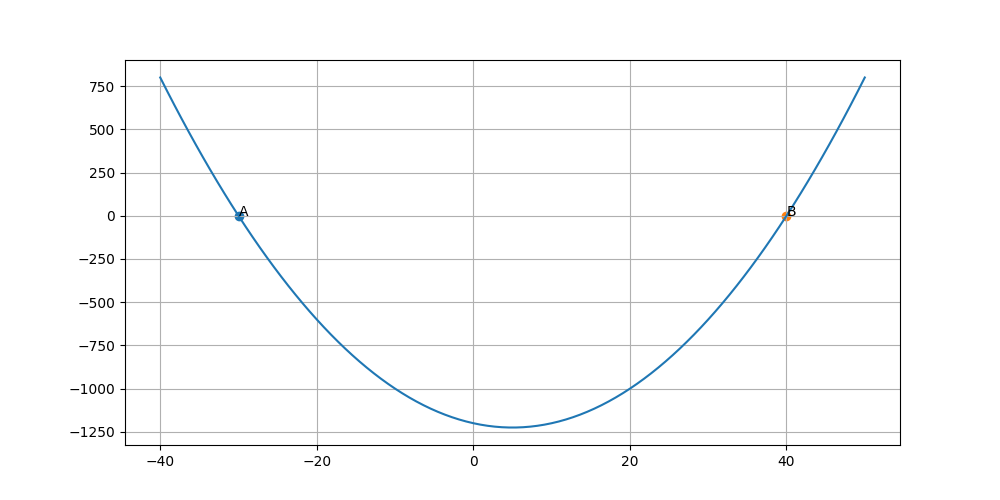
\includegraphics[width=\columnwidth]{a_4.png}
    \caption{}
    \label{a_4}
\end{figure}
\item The difference of two numbers is 5 and the difference of their reciprocals is $\displaystyle\frac{1}{10}$. Find the numbers.\\
 \solution \\
 \begin{align}
 & x - y =5  \label{5.11.1}\\
 & \dfrac{1}{x} - \dfrac{1}{y} = \dfrac{1}{10}\label{5.11.2}
 \end{align}
 Modifying equation \eqref{5.11.2}, we get
 \begin{align}
 &\dfrac{1}{x}-\dfrac{1}{x-5} = \dfrac{1}{10}\\
 &x^2-5x-50 = 0\\
 & x=10,-5\\
 &y = 5, -10
 \end{align}

  \begin{figure}[H]
	\centering
    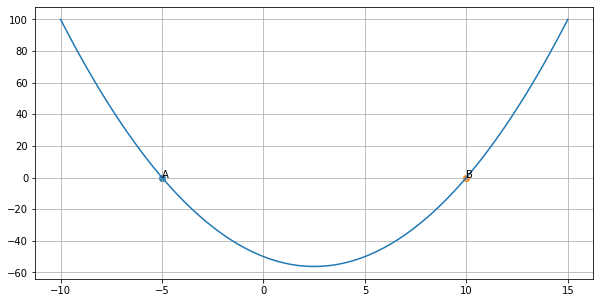
\includegraphics[width=\columnwidth]{l_10.png}
    \caption{}
    \label{l_10}
\end{figure}
\item Ms. Shahnaz earns Rs. 35,000 per month (excluding HRA). She donates Rs. 30,000 to Prime Minister Relief Fund (100\% exemption) and Rs. 40,000 to a Charitable Hospital (50\% exemption). She contributes Rs. 5,000 per month to Provident Fund and Rs. 25,000 per annum towards LIC premium. She purchases NSC worth Rs. 20,000. She pays Rs. 2,300 per month towards income tax for 11 month. Find the amount of income tax she has to pay in 12th month of the year.\\
Use the following to calculate income tax :
\begin{table}[ht]
    \begin{tabular}{p{0.45\columnwidth}p{0.45\columnwidth}}
    \textbf{(a) Saving:} & 100 \% exemption for permissible \\ & savings  upto Rs. 1,00,000 \\ \\
    \textbf{(b) Rates of income tax for ladies:} &\\ \\
    \textbf{Slab} & \textbf{Income tax} \\ \\
    (i) Upto Rs. 1,35,000 & No tax \\ 
    (ii) From Rs. 1,35,001 to Rs. 1,50,000 & 10\% of taxable income exceeding Rs. 1,35,000 \\ 
    (iii) From Rs. 1,50,001 to Rs. 2,50,000 & Rs. 1,500 + 20\% of the  amount excedding Rs. 1,50,000 \\
    (iv) From Rs. 2,50,001 and above & Rs. 21,500 + 30\% of the amount  exceeding Rs. 2,50,000 \\
    \textbf{Education Cess :} & 2\% of Income tax payable
    \end{tabular}
\end{table}\\
 \solution\\
 Annual Income = 35000 * 12 = Rs 420000\\
PF = 5000 * 12 = Rs 60000\\
LIC Premium = Rs 25000\\
NSC = Rs 20000\\
Saving Under 80C = 60000 + 25000 + 20000 = Rs 105000\\
Prime minister relief fund exemption = Rs  30000\\
Charitable hospital exemption = (50/100) * 40000 = Rs 20000\\
Total Donation exemption = 30000 + 20000 = Rs 50000\\
Taxable income = 420000 - 105000 - 50000 = Rs 265000\\
Tax Slab = 0-250000 =  0 \% \\
250000 - 50000 =  5 \% \\
265000 - 250000 = Rs 15000 \\
5\% of Rs 15000 = Rs 750 \\
Income tax already paid in 11 months = 2300 * 12 = Rs 27600\\ 
 \end{enumerate}
 \section{Trigonometry}
 \renewcommand{\theequation}{\theenumi}
\begin{enumerate}[label=\thesection.\arabic*.,ref=\thesection.\theenumi]
\numberwithin{equation}{enumi}
\item Prove that
 \begin{align}
 \displaystyle\frac{\cos A}{1-\tan A}+\displaystyle\frac{\sin A}{1-\cot A}=\sin A+\cos A \nonumber
 \end{align}
\solution \\
\begin{align}
& \displaystyle\frac{\cos A}{1-\tan A}+\displaystyle\frac{\sin A}{1-\cot A}=\sin A+\cos A 
\end{align}
\begin{align}
=& \displaystyle\frac{\cos A}{1-\tan A}+\displaystyle\frac{\sin A}{1-\cot A}\\
=& \displaystyle\frac{\cos A}{1-\tan A}+\displaystyle\frac{\sin A}{1-1/\tan A}\\
=& \displaystyle\frac{\cos A}{1-\tan A}+\displaystyle\frac{\sin A \tan A}{\tan A - 1}\\
=& \displaystyle\frac{\cos A}{1-\tan A} - \displaystyle\frac{\sin A \tan A}{1 - \tan A}\\
=& \displaystyle\frac{\cos A - \sin A \tan A}{1-\tan A}\\
=& \displaystyle\frac{\cos^2 A - \sin^2 A }{\cos A-\sin A}\\
=&\cos A+\sin A
\end{align}
\item Evaluate without using trigonometric tables :\\
 \bigskip
 $\displaystyle\frac{3\cos55\degree}{7\sin35\degree}+\displaystyle\frac{4(\cos70\degree.\cosec20\degree)}{7(\tan5\degree.\tan25\degree.\tan45\degree.\tan65\degree.\tan85\degree)}$
\solution \\ \\
 =$\displaystyle\frac{3\cos55\degree}{7\sin35\degree}+\displaystyle\frac{4(\cos70\degree.\cosec20\degree)}{7(\tan5\degree.\tan25\degree.\tan45\degree.\tan65\degree.\tan85\degree)}$\\ \\ \\
  =$\displaystyle\frac{3\cos(90- 35)\degree}{7\sin35\degree}+\displaystyle\frac{4(\cos70\degree.\cosec(90-70)\degree)}{7(\tan5\degree.\tan25\degree.\tan45\degree.\tan(90-25)\degree.\tan(90-5)\degree)}$\\ \\ \\
 =$\displaystyle\frac{3\sin35\degree}{7\sin35\degree}+\displaystyle\frac{4(\cos70\degree.\sec70\degree)}{7(\tan5\degree.\tan25\degree.\tan45\degree.\cot25\degree.\cot5\degree)}$\\ \\ 
 $=1$
 \item A boy standing on a horizontal plane finds a bird flying at a distance of 100 m from him at an elevation of 30$\degree$. A girl standing on the roof of 20 metre high building, finds the angle of elevation of the same bird to be 45$\degree$. Both the boy and the girl are on opposite sides of the bird. Find the distance of bird from the girl.\\
 \solution\\
 Given, \\  
\begin{table}[ht]
 \centering
 \resizebox{\columnwidth}{!}{
 \begin{tabular}{ |c|c|c| } 
 \hline
 Symbol & Description & Value\\
 \hline
$d_b$ & distance from bird to boy & 100m \\
 \hline
$\theta_b$ & elevation of bird from boy & $30\degree$ \\
 \hline
 $h_g$ & Height of girl from ground & 20m \\
 \hline
 $\theta_g$ & elevation of bird from girl & $45\degree$ \\
 \hline
 $d_g$ & distance of girl from bird & ? \\
 \hline
 $h$ & height of bird from ground & ?\\
 \hline
\end{tabular}}
 \caption{}
 \end{table}\\
\begin{align}
& h = d_b\tan \theta_b\\
& h = 100 \text{ x } 0.577= 57.7\\
& d_g = (h - h_b) /\tan \theta_g\\
& d_g = (57.7-20) \text{ x } 1 = 37.7
\end{align}
\begin{figure}[h!]
	\centering
    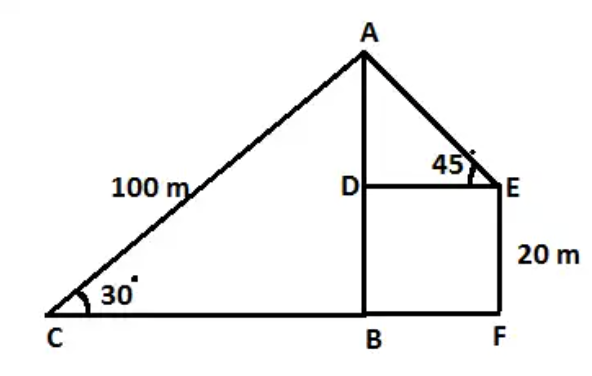
\includegraphics[width=0.75\columnwidth]{t_3.png}
    \caption{}
    \label{t_3}
\end{figure}
\end{enumerate}
\section{Linear Algebra}
 \renewcommand{\theequation}{\theenumi}
\begin{enumerate}[label=\thesection.\arabic*.,ref=\thesection.\theenumi]
\numberwithin{equation}{enumi}
\item solve the values of x and y.
\begin{align}
&x+\displaystyle\frac{6}{y}=6 & \\ 
&3x-\displaystyle\frac{8}{y}=5&
\end{align}
\solution Consider the equations  given in the problem statement.
\begin{align}
&x+\displaystyle\frac{6}{y}=6 \label{eq:0.0.3} &\\
&3x-\displaystyle\frac{8}{y}=5 \label{eq:0.0.4} &
\end{align}
The solution can be found by solving the above system of linear equations.\\ 
System of linear equations are defined as 
\begin{align}
\vec{Ax=B}\label{eq:0.0.5}
\end{align}
From the equations \eqref{eq:0.0.3} and \eqref{eq:0.0.4}, 
\begin{align}
&\vec{A}= \myvec{1 &6\\3  & -8}&\\
\medskip
&\vec{x}= \myvec{ x\\ \displaystyle\frac{1}{y}}&\\
\medskip
&\vec{B}= \myvec{6\\5} & 
\end{align} 
Substituting the values of $\vec{A}$, $\vec{x}$ and $\vec{B}$ in the equation \eqref{eq:0.0.5}
We get,
\begin{align}
\myvec{1&6\\3&-8} \myvec{x\\\displaystyle\frac{1}{y}}= \myvec{6\\5}
\end{align}
Considering the augmented matrix 
 \begin{align}
  &\myvec{1&6&6\\3&-8&5}&\\ 
& \xleftrightarrow[]{ R_2 \leftarrow R_2 - 3R_1}
  \myvec{1&6&6\\0&-26&-13}&\\
  & \xleftrightarrow[]{ R_1 \leftarrow 13R_1 + 3R_2}
  \myvec{13&0&39\\0&-26&-13}&\\
   & \xleftrightarrow[]{ R_1 \leftarrow R_1/3,R_2 \leftarrow R_2/-26}
  \myvec{1&0&3\\0&1&0.5}&
 \end{align}
 \begin{align}
&\myvec{1&0\\0&1} \myvec{x\\\displaystyle\frac{1}{y}}= \myvec{0\\0.5}& \label{eq:0.0.14}
\medskip
\end{align}
From the above equation \eqref{eq:0.0.14} we get,
\begin{align}
&x=3&\\
&y=2&
\end{align}
Therefore, x=3 and y= 2 are solutions to the given equations.
\item 
solve the values of x and y
\begin{align}
\displaystyle\frac{x+1}{2}+\displaystyle\frac{y-1}{3}=8\\
\displaystyle\frac{x-1}{3}+\displaystyle\frac{y+1}{2}=9\end{align}

\solution Consider the equations given in the problem statement.
\begin{align}
\displaystyle\frac{x+1}{2}+\displaystyle\frac{y-1}{3}=8\\
\displaystyle\frac{x-1}{3}+\displaystyle\frac{y+1}{2}=9
\end{align}
The above equations can be rearranged as the following equations
\begin{align}
3x+2y=47 \label{eq:0.0.21}\\
2x+3y=53 \label{eq:0.0.22}
\end{align}
The solution can be found by solving the above system of linear equations.\\ 
System of linear equations are defined as 
\begin{align}
\vec{Ax=B} \label{eq:0.0.23}
\end{align}
From the equations \eqref{eq:0.0.21} and \eqref{eq:0.0.22}, 
\begin{align}
&\vec{A}= \myvec{3 &2\\2 & 3}&\\
\medskip
&\vec{x}= \myvec{ x\\ y}&\\
\medskip
&\vec{B}= \myvec{47\\53}&  
\end{align} 
Substituting the values of $\vec{A}$, $\vec{x}$ and $\vec{B}$ in the equation \eqref{eq:0.0.23}
We get,
\begin{align}
&\myvec{3&2\\2&3} \myvec{x\\y}= \myvec{47\\53}&
\end{align}
Considering the augmented matrix 
 \begin{align}
& \myvec{3&2&47\\2&3&53}&
 \\
&\xleftrightarrow[]{ R_2 \leftarrow 3R_2 - 2R_1}
 \myvec{3&2&47\\0&5&65}&\\
 &\xleftrightarrow[]{ R_1 \leftarrow 5R_1 - 2R_2}
 \myvec{15&0&105\\0&5&65}&\\
 &\xleftrightarrow[]{ R_1 \leftarrow R_1/15,R_2\leftarrow R_2/5}
 \myvec{1&0&7\\0&1&13}&
 \end{align}
 \begin{align}
&\myvec{1&0\\0&1} \myvec{x\\y}= \myvec{7\\13}& \label{eq:0.0.32}
\medskip
\end{align}
By solving equation \eqref{eq:0.0.32} we get,
\begin{align}
&x=7&\\
&y= 13&
\end{align}
Therefore, x=7 and y= 13 are solutions to the given equations. 
\begin{figure}[H]
	\centering
    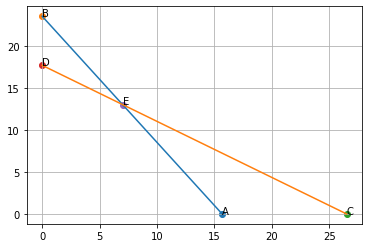
\includegraphics[width=\columnwidth]{l_5.png}
    \caption{}
    \label{l_5}
\end{figure}
\item  Show that the points given below are vertices of an isosceles right angle triangle.
\begin{align}
\myvec{7\\10}, \myvec{-2\\5} \text{and} \myvec{3\\-4}
\end{align}

\solution Consider the given points as vectors,
\begin{align}
&\vec{A}= \myvec{7\\10}&\\
&\vec{B}=\myvec{-2\\5}&\\
&\vec{C}=\myvec{3\\-4}&
\end{align}
For a triangle to be an isosceles, any two sides of the triangle should be equal.
For finding a triangle to be isosceles and right angle, we consider,
\begin{align}
&\vec{A-B}= \myvec{7\\10} - \myvec{-2\\5} = \myvec{9\\5}&\\
&\vec{B-C}= \myvec{-2\\5} - \myvec{3\\-4} = \myvec{-5 \\ 9}&\\
&\vec{C-A}=  \myvec{3\\-4} - \myvec{7\\10} = \myvec{-4\\ -14}&
\end{align}
\begin{align}
&\vec{(A-B)}^T\vec{(B-C)} = \myvec{9&5}\myvec{-5\\9} &\\&= -45+45 = 0 \label{eq:0.0.43}&\\
& \vec{(C-A)}^T\vec{(A-B)} = \myvec{-4&-14}\myvec{9\\5}&\\& = -36-70 = -106 \label{eq:0.0.45}&\\
 &\vec{(B-C)}^T\vec{(C-A)} = \myvec{-5&9}\myvec{-4\\-14}&\\& = 20-126 = -106 \label{eq:0.0.47}&
\end{align}
From the equation \eqref{eq:0.0.43} \begin{align} \vec{A-B} \perp \vec{B-C}\end{align} Therefore $\measuredangle{B} = 90\degree$.
From the equations \eqref{eq:0.0.45} and \eqref{eq:0.0.47} $\measuredangle{CAB}=\measuredangle{BCA}$.
Therefore, $\triangle{ABC}$ is an isosceles right angle triangle with sides AB=BC and right angle at B.
\bigskip
\begin{figure}[H]
	\centering
    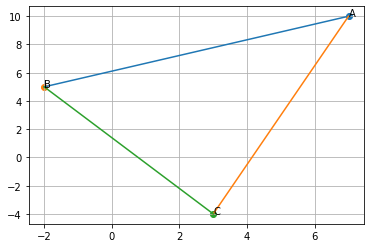
\includegraphics[width=\columnwidth]{l_6.png}
    \caption{}
    \label{l_6}
\end{figure}
\item In what ratio does the line \begin{align} \myvec{1&-1}\vec{x}=2 \label{eq:0.0.49}\end{align} divides the line segment joining \begin{align}\myvec{3 \\-1} \text{and} \myvec{8\\9} \label{eq:0.0.50}\end{align}

\solution Consider the line \begin{align} \vec{n}^T\vec{x}=c \end{align} divides the line segment $\vec{A}$ and $\vec{B} $ in $k:1$ ratio.
$\vec{p} $ is point of intersection of two lines.\\ 
From the section formula we can write,
\begin{align}
&\vec{p} = \displaystyle\frac{1}{k+1}\left[\vec{A}+ k\vec{B}\right]&\\
 \end{align}
The point $\vec{p}$ passes through the line $\vec{n}^T\vec{x}=c$, therefore,
\begin{align}
&\vec{n}^T\vec{p}=c&\\
&\vec{n}^T\left(\displaystyle\frac{\vec{A}+k\vec{B}}{k+1} \right)=c&
\end{align}
Solving for k, we get,
\begin{align}
&k=\displaystyle\frac{c-\vec{n}^T\vec{A}}{\vec{n}^T\vec{B}-c} \label{eq:0.0.56} &
\end{align}
From the equations \eqref{eq:0.0.49} and \eqref{eq:0.0.50},
\begin{align}
& \vec{n}^T = \myvec{1&-1}&\\
& \vec{A} = \myvec{3 \\-1}&\\
& \vec{B} = \myvec{8\\9}
\end{align}
Substituting the above values in the equation \eqref{eq:0.0.56}, we get,
\begin{align}
& k = \displaystyle\frac{2-\myvec{1&-1}\myvec{3\\-1}}{\myvec{1&-1}\myvec{8\\9} - 2}&\\
&k = \displaystyle\frac{2}{3}
\end{align}
Therefore, the line \begin{align} \myvec{1&-1}\vec{x}=2 \end{align} divides the line segment joining \begin{align}\myvec{3 \\-1} \text{and} \myvec{8\\9} \end{align} in 2:3 ratio.
\begin{figure}[H]
	\centering
    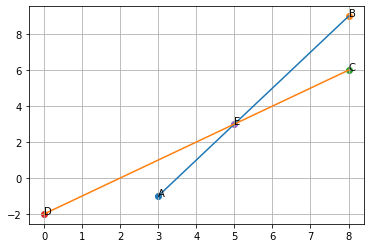
\includegraphics[width=\columnwidth]{l_7.png}
    \caption{}
    \label{l_7}
\end{figure}
\item $\vec{P}$  and $\vec{Q}$ are points on the sides $\vec{CA}$ and $\vec{CB}$ respectively of $\triangle{ABC}$, right angled at C. Prove that
\begin{align}
&\vec{AQ}^2+ \vec{BP}^2= \vec{AB}^2+\vec{PQ}^2 \label{eq:5.1}
\end{align}
\solution construction of figure. \\
Input parameters and output parameters are shown in the table \ref{1}.\\
\begin{table}[htb]
 \centering
 \resizebox{\columnwidth}{!}{
 \begin{tabular}{ |c|c|c| } 
 \hline
 Symbol & Description & Value\\
 \hline
 $\vec{B}$ & vertex B & $\myvec{0\\0}$ \\
 \hline
c & length of the side opposite to vertex C & 5cm \\
 \hline
$\theta_B$ & angle at vertex B & $30\degree$ \\
 \hline
 $k_1$ & Ratio of point Q diving the line CB& 2 \\
 \hline
 $K_2$ & Ratio of point P diving the line CA & $3$ \\
 \hline
\end{tabular}}
 \caption{Input Parameters}
 \label{1}
 \end{table}
 
 \begin{table}[htb]
 \centering
 \resizebox{\columnwidth}{!}{
 \begin{tabular}{ |c|c|c| } 
 \hline
 Symbol & Description & Value\\
 \hline
 $\vec{A}$ & vertex A & $\myvec{b\cos B\\b\sin B}$ \\
 \hline
$\vec{C}$ & vertex C & $\myvec{b\cos B\\ 0}$ \\
 \hline
 $\vec{P} $& vertex P & $\myvec{b\cos B\\K_2}$ \\
 \hline
 $\vec{Q}$ & vertex Q & $\myvec{K_1\\0}$ \\
 \hline
\end{tabular}}
 \caption{Output Parameters}
 \label{tab:1}
 \end{table}
 \begin{figure}[H]
	\centering
    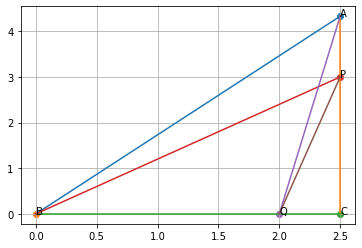
\includegraphics[width=\columnwidth]{l_1.png}
    \caption{}
    \label{l_1}
\end{figure}
From the python code, \eqref{eq:5.1} is proved.
 \item In figure \ref{l_2} , $\vec{DE} $ $\|$ $\vec{AB} $ and $\vec{FE} $ $\|$ $\vec{DB} $. Prove that 
\begin{align}
\vec{DC}^2=\vec{CF}.\vec{AC} \label{eq:5.2}
\end{align}
\solution Construction of the figure,\\
Input parameters and output parameters are shown in the table \ref{2}\\
\begin{table}[htb]
 \centering
 \resizebox{\columnwidth}{!}{
 \begin{tabular}{ |c|c|c| } 
 \hline
 Symbol & Description & Value\\
 \hline
 $\vec{A}$ & vertex $\vec{A}$ & $\myvec{0\\0}$ \\
 \hline
c & length of the side opposite to vertex C & 3cm \\
 \hline
 b & length of the side opposite to vertex B & 5cm \\
 \hline
$\theta_A$ & angle at vertex $\vec{A}$ & $30\degree$ \\
 \hline
 k & Ratio of point D diving the line AC& 2 \\
 \hline
\end{tabular}}
 \caption{Input Parameters}
 \label{2}
 \end{table}
 
 \begin{table}[htb]
 \centering
 \resizebox{\columnwidth}{!}{
 \begin{tabular}{ |c|c|c| } 
 \hline
 Symbol & Description & Value\\
 \hline
 $\vec{C}$ & vertex C & $\myvec{b\cos B\\b\sin B}$ \\
 \hline
$\vec{B}$ & vertex B & $\myvec{c\\ 0}$ \\
 \hline
$ \vec{D}$ & vertex D & $\dfrac{K\vec{A}+\vec{C}}{k+1}$ \\
 \hline
 $ \vec{E}$ & vertex E & $\dfrac{K\vec{B}+\vec{C}}{k+1}$ \\ 
 \hline
  $ \vec{F}$ & vertex F & $\dfrac{K\vec{D}+\vec{C}}{k+1}$ \\
   \hline
\end{tabular}}
 \caption{Output Parameters}
 \label{tab:2}
 \end{table}
\begin{figure}[H]
	\centering
    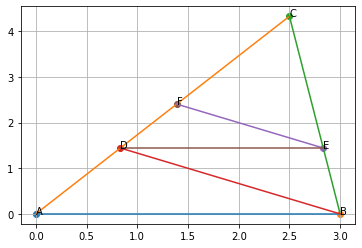
\includegraphics[width=\columnwidth]{l_2.png}
    \caption{}
    \label{l_2}
\end{figure}
From the python code, \eqref{eq:5.2} is proved.
\item Solve the following system of equations graphically :
\begin{align}
&2X+3Y=8\nonumber \\ &X+4Y=9 \nonumber
\end{align}
\solution\\
Consider the equations,
\begin{align}
&2X+3Y=8  \label{eq:21} \\
&X+4Y=9 \label{eq:22}
\end{align}
The solution can be found by solving the above system of linear equations.\\ 
System of linear equations are defined as 
\begin{align}
\vec{Ax=B} \label{eq:23}
\end{align}
From the equations \eqref{eq:21} and \eqref{eq:22}, 
\begin{align}
&\vec{A}= \myvec{2 &3\\1 & 4}&\\
\medskip
&\vec{x}= \myvec{ x\\ y}&\\
\medskip
&\vec{B}= \myvec{8\\9}&  
\end{align} 
Substituting the values of $\vec{A}$, $\vec{x}$ and $\vec{B}$ in the equation \eqref{eq:23}
We get,
\begin{align}
&\myvec{2&3\\1&4} \myvec{x\\y}= \myvec{8\\9}&
\end{align}
Considering the augmented matrix 
 \begin{align}
& \myvec{2&3&8\\1&4&9}&
 \\
&\xleftrightarrow[]{ R_2 \leftarrow 2R_2 - R_1}
 \myvec{2&3&8\\0&5&10}&\\
 &\xleftrightarrow[]{ R_1 \leftarrow 5R_1 - 3R_2}
 \myvec{10&0&10\\0&5&10}&\\
 &\xleftrightarrow[]{ R_1 \leftarrow R_1/10,R_2\leftarrow R_2/5}
 \myvec{1&0&1\\0&1&2}&
 \end{align}
 \begin{align}
&\myvec{1&0\\0&1} \myvec{x\\y}= \myvec{1\\2}& \label{eq:32}
\medskip
\end{align}
By solving equation \eqref{eq:32} we get,
\begin{align}
&x=1&\\
&y= 2&
\end{align}
Therefore, x=1 and y= 2 are solutions to the given equations.
\begin{figure}[H]
	\centering
    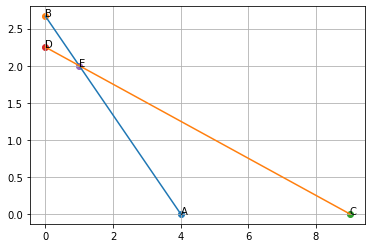
\includegraphics[width=\columnwidth]{l_3.png}
    \caption{}
    \label{l_3}
\end{figure}
\item In figure, \ref{l_4} $\vec{TA}$ is a tangent to the circle from a point T and $\vec{TBC}$ is a secant to the circle. If $\vec{AD}$ is the bisector of $\measuredangle{CAB} $, prove that $\triangle{ADT} $ is isosceles.\\
\solution \\
Input parameters,\\
\begin{table}[htb]
 \centering
 \resizebox{\columnwidth}{!}{
 \begin{tabular}{ |c|c|c| } 
 \hline
 Symbol & Description & Value\\
 \hline
 $\vec{O}$ & center of the circle & $\myvec{0\\0}$ \\
 \hline
r & radius of the circle & 2cm \\
 \hline
 d & distance of point $\vec{T}$ & 5cm \\
 \hline
$\beta$ & $\measuredangle{OTB}$ & $20\degree$ \\
 \hline
 $\vec{T}$ & Point $\vec{T}$ & $\myvec{5\\0}$ \\
 \hline
\end{tabular}}
 \caption{Input Parameters}
 \label{3}
 \end{table}
From the figure \ref{l_4},
\begin{align}
& \vec{T} = \myvec{d,0}\\
& \measuredangle{OTA} = \sin^{-1}\left(\dfrac{\|OA\|}{\|OT\|}
\right)\\
&\measuredangle{OTA} = \sin^{-1}\left(\dfrac{2}{5}\right) = 23.57\degree 
\end{align} 
Finding the coordinates of $\vec{A}$.\\
Equation of line $\vec{AT}$ is given by,
\begin{align}
& \vec{x} = \vec{T} +\lambda\vec{m} \label{5.7.1}
\end{align}
where m is the the directional vector, $\vec{m} = \myvec{1\\ m }$, where m is slope of the line.
\begin{align}
& m=\tan \measuredangle{180 - OTA} = -0.436\\
& \vec{x} = \myvec{5\\0} +\lambda\myvec{1\\-0.436}
\end{align}
Point $\vec{A} $is intersection of circle and tanget $\vec{AT}.$\\
Equation of the circle,
\begin{align}
& \vec{x}^T\vec{A}\vec{x} +2\vec{b}^T\vec{x}+c=0\\ \label{5.7.2}
&\vec{A} = \myvec{1&0\\0&1}\\
&\vec{b} = \myvec{0\\0}\\
&c = -4
\end{align}
From \eqref{5.7.1} and \eqref{5.7.2},
\begin{align}
& \vec{x}^T\vec{A}\vec{x} +2\vec{b}^T\vec{x}+c=0\\
& \vec{x} = \vec{T} +\lambda\vec{m} \\
& \vec{T+\lambda\vec{m}}^T\vec{A}\vec{T+\lambda\vec{m}} +2\vec{b}^T \vec{T+\lambda\vec{m}}+c = 0 \\
& \vec{T+\lambda\vec{m}^T}\vec{A}\vec{T+\lambda\vec{m}} +2\vec{b}^T \vec{T+\lambda\vec{m}}+c = 0
\end{align}
Substituting the values of $\vec{A}$ and $\vec{b}$ we get,
\begin{align}
& \|\vec{T}\|^2+2\lambda(\vec{m}^T\vec{T})+\lambda^2\|\vec{m}\|^2+c = 0 \\
& \lambda^2\|\vec{m}\|^2 +2\lambda(\vec{m}^T\vec{T}) + \|\vec{T}\|^2 + c = 0
\end{align}
Substituting the values of $\vec{T}$ and $\vec{m}$,
\begin{align}
&1.19\lambda^2 +10\lambda +21 = 0\\
&\lambda = -4.2,-4.2
\end{align}
Substituting the lambda value in \eqref{5.7.1} we get,
\begin{align}
& \vec{A} = \vec{T} +\lambda\vec{m}\\
& \vec{A} = \myvec{5\\0} -4.2\myvec{1\\-0.436}\\
& \vec{A} = \myvec{0.8\\1.831}
\end{align}
Finding the coordinates of $\vec{B}$ and $\vec{C}$.\\
$\measuredangle{OTB}$ is $< \measuredangle{OTA}$. Therefore, select $\measuredangle{OTB} = 20\degree$. Using the equations \eqref{5.7.1} and \eqref{5.7.2}. Here the direction vector $\vec{m}$ is $\myvec{1\\0.363}$.\\
\begin{align}& \vec{x} = \myvec{5\\0} +\lambda\myvec{1\\0.363}\end{align}
Equation of the circle,
\begin{align}
& \vec{x}^T\vec{A}\vec{x} +2\vec{b}^T\vec{x}+c=0\\ \label{5.7.2-second}
&\vec{A} = \myvec{1&0\\0&1}\\
&\vec{b} = \myvec{0\\0}\\
&c = -4
\end{align}
\begin{align}
& \vec{x}^T\vec{A}\vec{x} +2\vec{b}^T\vec{x}+c=0\\
& \vec{x} = \vec{T} +\lambda\vec{m} \\
& \vec{T+\lambda\vec{m}}^T\vec{A}\vec{T+\lambda\vec{m}} +2\vec{b}^T \vec{T+\lambda\vec{m}}+c = 0 \\
& \vec{T+\lambda\vec{m}^T}\vec{A}\vec{T+\lambda\vec{m}} +2\vec{b}^T \vec{T+\lambda\vec{m}}+c = 0
\end{align}
Substituting the values of $\vec{A}$ and $\vec{b}$ we get,
\begin{align}
& \|\vec{T}\|^2+2\lambda(\vec{m}^T\vec{T})+\lambda^2\|\vec{m}\|^2+c = 0 \\
& \lambda^2\|\vec{m}\|^2 +2\lambda(\vec{m}^T\vec{T}) + \|\vec{T}\|^2 + c = 0
\end{align}
Substituting the values of $\vec{T}$ and $\vec{m}$,
\begin{align}
&1.13\lambda^2 +10\lambda +21 = 0\\
&\lambda = -3.42,-5.42
\end{align}
Substituting the lambda value in \eqref{5.7.1} we get,
\begin{align}
& \vec{x} = \vec{T} +\lambda\vec{m}\\
& \vec{C} = \myvec{5\\0} -3.42\myvec{1\\0.363}\\
& \vec{C} = \myvec{1.58\\-1.241}\\
& \vec{B} = \myvec{5\\0} -5.42\myvec{1\\0.363}\\
& \vec{B} = \myvec{-0.42\\1.96}
\end{align}
Finding the coordinates of $\vec{D}$.\\
$\vec{AD}$ is the angular bisector of $\measuredangle{BAC}$.\\
Equation of angular bisector,\\
\begin{align}
&\dfrac{\vec{n_1}^T\vec{x}+c_1}{\|n_1\|} = \pm \dfrac{\vec{n_2}^T\vec{x}+c_2}{\|n_2\|} \label{5.7.3}
\end{align}
where,
$\vec{n_1}^T\vec{x}+c_1$ is the equation of line $\vec{AB}$ and $\vec{n_2}^T\vec{x}+c_2$ is the equation of line $\vec{AC}$.
Equation of line $\vec{AB}$,
\begin{align}
& \vec{n_1}^T\vec{x-A} = 0\\
& \myvec{3.99&1}\vec{x} = 5.02
\end{align}
Equation of line $\vec{AC}$,
\begin{align}
& \vec{n_2}^T\vec{x-A} = 0\\
& \myvec{3.21&-1}\vec{x} = 0.72
\end{align}
 From equation \eqref{5.7.3} of angular bisector we get, 
\begin{align}
& \dfrac{\myvec{3.99&1}\vec{x}-5.02}{\|\myvec{3.99\\1}\|} = \pm \dfrac{ \myvec{3.21&-1}\vec{x}-0.72}{\|\myvec{3.21\\-1}\|} \label{5.7.4}
\end{align}
Solving equation \eqref{5.7.4}, we get 2 equations  of angular bisectors
\begin{align}
&  \myvec{0.211&7.476}\vec{x}-13.916 = 0 \label{5.7.5}\\
&\myvec{26.619&0.751}\vec{x}-19.84 = 0 \label{5.7.6}
\end{align}
From the equations \eqref{5.7.5} and \eqref{5.7.6}, only \eqref{5.7.6} forms point $\vec{D}$, intersection of $\vec{AD}$ and $\vec{TBC}$
\begin{align}
&\vec{AD} = \myvec{26.619&0.751}\vec{x}-19.84 = 0 \label{5.7.7} \\
&\vec{TBC} =\myvec{0.36&-1}\vec{x}-1.81 = 0 \label{5.7.8}
\end{align} 
Solving \eqref{5.7.7} and \eqref{5.7.8}, we get
\begin{align}
\vec{D} = \myvec{0.703\\-1.556}
\end{align}
Proof of $\triangle ADT$ being an isosceles is done using python code
\begin{figure}[H]
	\centering
    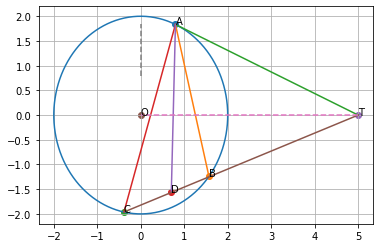
\includegraphics[width=\columnwidth]{l_4.png}
    \caption{}
    \label{l_4}
\end{figure}
\item In  the $\triangle{ABC}$, $\vec{AD} \perp \vec{BC}$ and $\vec{AD^2}= \vec{BD}.\vec{DC}$.  Prove that $\measuredangle{BAC}$ is a right angle.\\
\solution\\
Consider,
\begin{table}[htb]
 \centering
 \resizebox{\columnwidth}{!}{
 \begin{tabular}{ |c|c|c| } 
 \hline
 Symbol & Description & Value\\
 \hline
 $\vec{B}$ & vertex $\vec{A}$ & $\myvec{0\\0}$ \\
 \hline
c & length of the side opposite to vertex C( $\vec{AB}$) & 5cm \\
 \hline
$\theta_B$ &  $\measuredangle{ABC}$ & $60\degree$ \\
 \hline
\end{tabular}}
 \caption{}
 \label{table:2}
 \end{table}
 Given, \begin{align} \vec{AD}^2 = \vec{BD}\vec{CD} \end{align}
 From the figure \ref{l_8}, we get
 \begin{align}
 & \|AD\| = c\sin \theta_B = 5\sin 30\degree \\
 & \|BD\| = c\cos \theta_B = 5\cos 30\degree\\
 & \|DC\| = \dfrac{\|AD\|^2}{\|BD\|}\\
 & \|BC\| = \|BD\| + \|DC\| \\
 &\vec{A} = \myvec{-c\\0} = \myvec{-5\\0}\\
 & \vec{D} = \myvec{-\|BD\|\cos \theta_B \\ \|BD\|\sin \theta_B }\\
 & \vec{C} = \myvec{-\|BC\|\cos \theta_B \\ \|BC\|\sin \theta_B}
 \end{align}
 \begin{figure}[H]
	\centering
    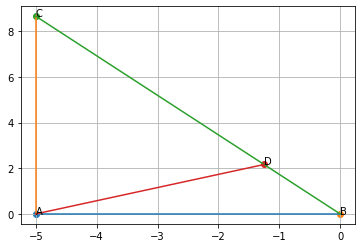
\includegraphics[width=\columnwidth]{l_8.png}
    \caption{}
    \label{l_8}
\end{figure}
Proof that $\measuredangle{CAB}$ is right angle is done in python
\item If a line is drawn parallel to one side of a triangle, to intersect the other two sides in distinct points, prove that the other two sides are divided in the same ratio.\\ Figure, $\ref{l_9}$ $\vec{DE} \| \vec{BC}$ and $\vec{BD}=\vec{CE}$. Prove that $\triangle{ABC}$ is an isosceles triangle.\\
\solution \\
Consider,
\begin{table}[htb]
 \centering
 \resizebox{\columnwidth}{!}{
 \begin{tabular}{ |c|c|c| } 
 \hline
 Symbol & Description & Value\\
 \hline
 $\vec{A}$ & vertex $\vec{A}$ & $\myvec{0\\0}$ \\
 \hline
c & length of the side opposite to vertex C( $\vec{AB}$) & 5cm \\
 \hline
 a & length of the side opposite to vertex A( $\vec{BC}$) & 4cm \\
 \hline
$\theta_B$ &  $\measuredangle{ABC}$ & $60\degree$ \\
 \hline
  $k$ & Ratio of point $\vec{P}$ and $\vec{Q}$ diving the line $\vec{AB}$ and $\vec{AC}$ respectively & 2 \\
 \hline
\end{tabular}}
 \caption{}
 \label{tab:dup-2}
 \end{table}
 Given, two sides $\vec{AB}$ and$\vec{AC}$ are divided equally by the points $\vec{P}$ and $\vec{Q}$. Let K is the ratio.\\
 \begin{align}
 &\vec{P} = \dfrac{K\vec{A}+\vec{C}}{k+1}\\
 &\vec{Q} = \dfrac{K\vec{A}+\vec{B}}{k+1}
 \end{align}
 Given $\vec{A} = \myvec{0\\0}$, c=5, a = 4 and $\measuredangle{CAB} = 60\degree$ 
 \begin{align}
 &\vec{B} = \myvec{a\\0} = \myvec{4,0}\\
 &\vec{C} = \myvec{c\cos \measuredangle{CAB}\\ c\sin \measuredangle{CAB}} = \myvec{5 \cos 60\degree\\5\sin 60\degree}
 \end{align}
\begin{figure}[H]
	\centering
    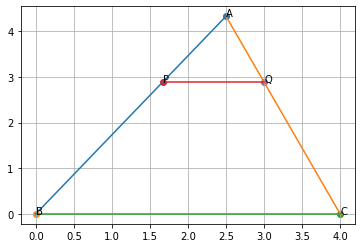
\includegraphics[width=\columnwidth]{l_9.png}
    \caption{}
    \label{l_9}
\end{figure}
Proof of $\triangle{ABC}$ is isosceles done in python code.\\

 \end{enumerate}
\section{Probability and statastics}
\renewcommand{\theequation}{\theenumi}
\begin{enumerate}[label=\thesection.\arabic*.,ref=\thesection.\theenumi]
\numberwithin{equation}{enumi}
\item The mean of the following frequency distribution is 62.8. Find the missing frequency x.
\\
\begin{table}[ht]
 \centering
 \resizebox{\columnwidth}{!}{
 \begin{tabular}{ |c|c|c|c|c|c|c| } 
 \hline
 Class & 0-20 & 20-40 & 40-60 & 60-80 & 80-100 & 100-120\\
 \hline
Frequency & 5 & 8 & x & 12 & 7 & 8\\
 \hline
\end{tabular}}
 \caption{}
 \end{table}
 \solution\\
 \begin{table}[ht]
 \centering
 \resizebox{\columnwidth}{!}{
 \begin{tabular}{ |c|c|c|c|c|c|c| } 
 \hline
 Class & 0-20 & 20-40 & 40-60 & 60-80 & 80-100 & 100-120\\
 \hline
Frequency & 5 & 8 & x & 12 & 7 & 8\\
 \hline
 $x_i$ &10&30&50&70&90&110\\
 \hline
 $f_ix_i$& 50&240&50x&840&630&880\\
 \hline
\end{tabular}}
 \caption{}
 \end{table}
 let
 \begin{align}
 &\vec{fx} = \myvec{50\\240\\840\\630\\880}\\
 &\vec{f} = \myvec{5\\8\\12\\7\\8} 
 \end{align}
 \begin{align}
 &E(x) = \dfrac{\vec{1}^T\vec{fx}+50x}{\vec{1}^T\vec{f}+x}\\
 & x =\dfrac{E(x)(\vec{1}^T\vec{f})-\vec{1}^T\vec{fx}}{50-E(x)}\\
 &62.8 = \dfrac{2640+50x}{40+x}\\
 & x = 10 
 \end{align}
 \item Cards marked with numbers 3, 4, 5, ......, 50 are placed in a box and mixed thoroughly. One card is drawn at random from the box. Find the probability that number on the drawn card is
\begin{enumerate}
\item divisible by 7.
\item a number which is a perfect square.
\end{enumerate}
\solution\\
Let A = numbers divisible by 7.\\
\begin{align}
\{A\} = {7,14,21,28,35,42,49}\\
\{S\} = {3,4,5, ...,50}\\
n(A) = 9\\
n(S) = 48\\
P(A) =\dfrac{n(A)}{n(S)} = \dfrac{9}{48}
\end{align}
Let B = a number which is a perfect square.\\
\begin{align}
\{B\} = {4,9,16,25,36,49}\\
\{S\} = {3,4,5, ...,50}\\
n(B) = 6\\
n(S) = 48\\
P(B) =\dfrac{n(B)}{n(S)} = \dfrac{6}{48}
\end{align}
\item The enrolment of a secondary school in different classes is given below. Draw a pie chart to represent the above data.\\
 \begin{table}[htb]
 \centering
 \resizebox{\columnwidth}{!}{
 \begin{tabular}{ |c|c|c|c|c|c| } 
 \hline
 Class & VI & VII & VIII & IX & X \\
 \hline
Enrolment & 600 & 500 & 400 & 700 & 200\\
 \hline
\end{tabular} }
 \caption{}
 \end{table}
\solution\\
\begin{figure}[H]
	\centering
    \includegraphics[width=\columnwidth]{P_1.png}
    \caption{}
    \label{P_1}
\end{figure}
 \item A bag contains 5 red balls and some blue balls. If the probability of drawing a blue ball from the bag is thrice that of a red ball, find the number of blue balls in the bag.\\
 \solution\\
 Let X be a random variable, X= No. of balls\\
 X=0 is no.of red balls\\
 X=1 is no. of blue balls\\
 Let s be total no.of balls.\\
 Given,
 \begin{align}
 &P_X(x=0) = \dfrac{5}{s}\\
 &P_X(x=1) = \dfrac{s-5}{s}\\
 &P_X(x=1) = 3P_X(x=0)\\
 &\dfrac{s-5}{s} =  \dfrac{15}{s}\\
 &s=20
 \end{align}
 Therefore no.of blue balls are 15.
\end{enumerate}
\end{document}
